\documentclass[a4paper,12pt]{article}

\usepackage [utf8x] {inputenc} %кодировка исходного текста
\usepackage [T2A] {fontenc} %кодировка
\usepackage [english, russian] {babel}
\usepackage{color}
\usepackage{amsmath, amsfonts, amssymb, amsthm, mathtools}
\usepackage{graphicx}
\graphicspath{{.}}
\DeclareGraphicsExtensions{.pdf,.png,.jpg}
\righthyphenmin=2


\title{Мечтают ли андроиды об электроовцах?}
\author{Филип К. Дик}
\date{1968}


\begin{document}


\begin{figure}[h] % так вставляются скриншоты с кодом и его выводом
		\centering
			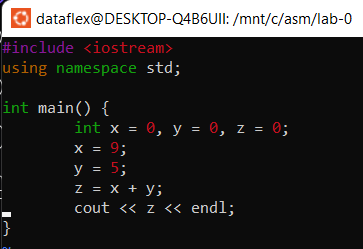
\includegraphics[width=0.8\linewidth]{arithmetic cpp.png}
\end{figure}


\begin{figure}[h] % так вставляются скриншоты с кодом и его выводом
		\centering
			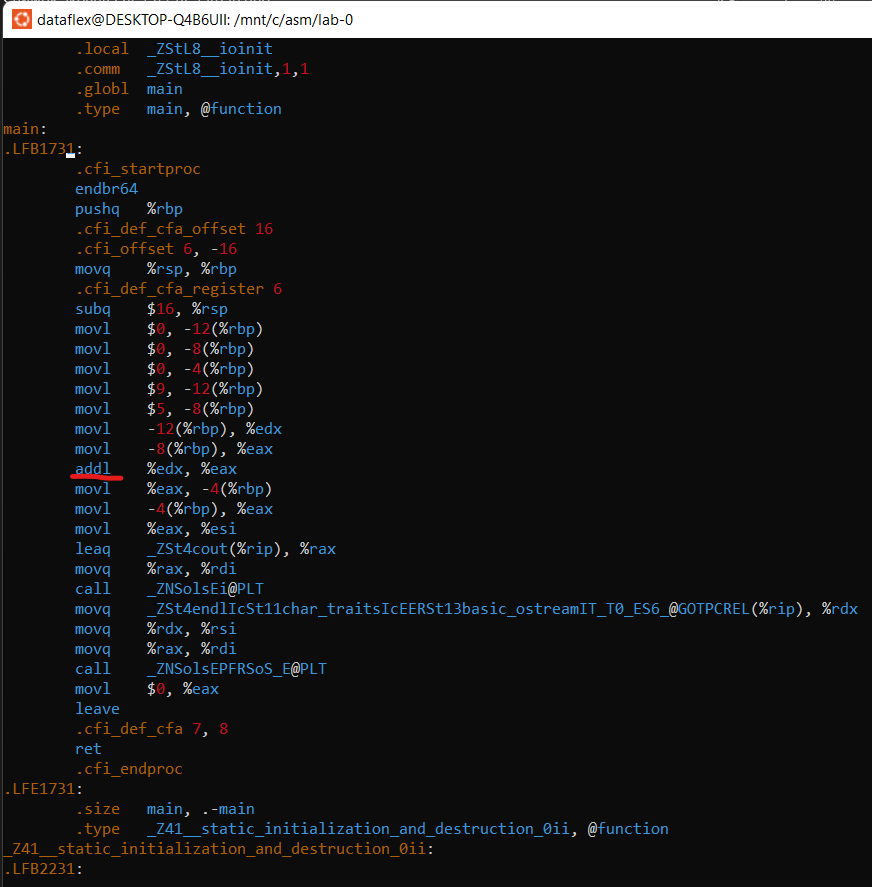
\includegraphics[width=0.8\linewidth]{arithmetic add.png}
\end{figure}


\begin{figure}[h] % так вставляются скриншоты с кодом и его выводом
		\centering
			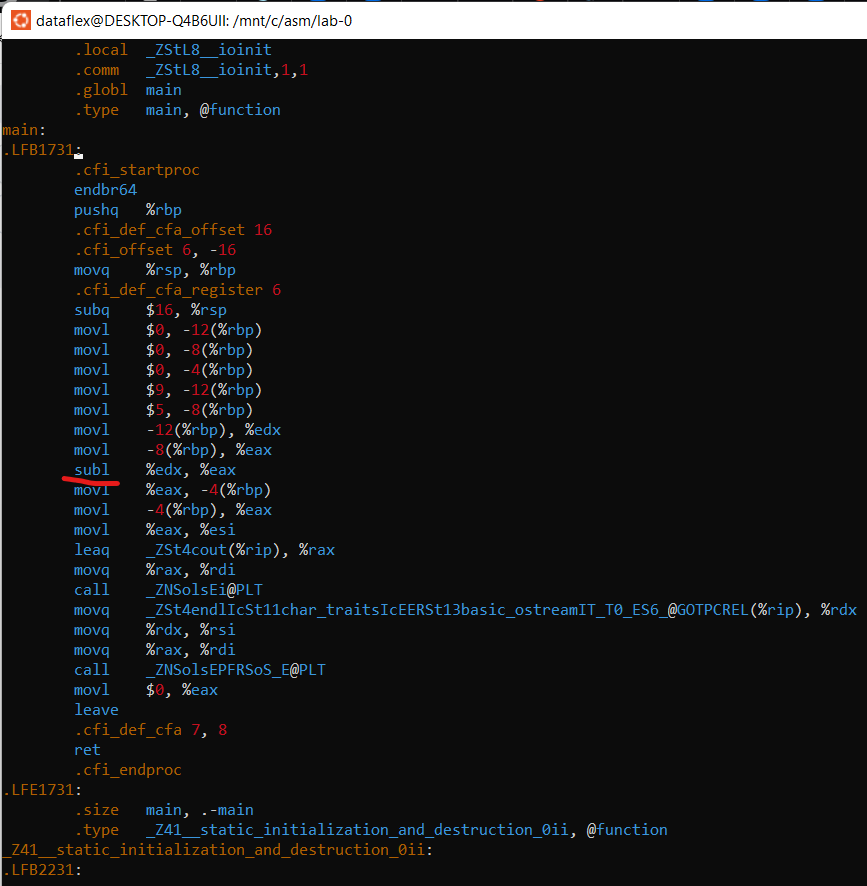
\includegraphics[width=0.8\linewidth]{arithmetic sub.png}
\end{figure}


\begin{figure}[h] % так вставляются скриншоты с кодом и его выводом
		\centering
			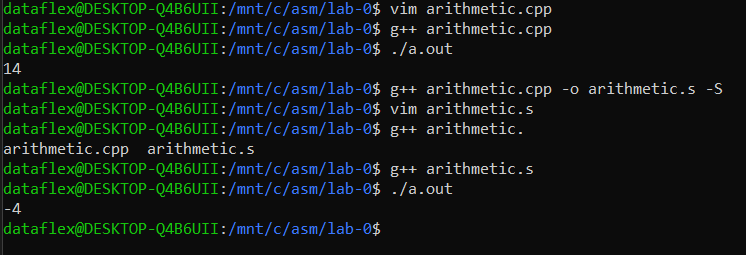
\includegraphics[width=0.8\linewidth]{arithmetic command line.png}
\end{figure}

\begin{table}[h] % ни в коем случае верстать таблицы вручную -- для этого есть https://www.tablesgenerator.com/
  \centering
  \begin{tabular}{|c|c|c|}
  \hline
  x & o &  \\ \hline
  o & x &  \\ \hline
  o &  & x \\ \hline
  \end{tabular}
\end{table}

\end{document}
